\apendice{Especificación de diseño}

\section{Introducción}
En este apartado se van a explicar elementos del diseño del proyecto que explican su funcionamiento y estructura.

\section{Trabajo propio vs trabajo ajeno}
Antes de nada es necesario mencionar que este trabajo ha partido de una platilla que ofrece Unity como punto de partida. Esa plantilla se llama Platformer Microgame y se puede añadir a tus assets en el siguiente enlace:\\
 \url{https://assetstore.unity.com/packages/templates/platformer-microgame-151055?_gl=1*cat3jy*_ga*NTAyOTIzMjY4LjE2MTIzNTE0Nzk.*_ga_1S78EFL1W5*MTYyMzE0MTIwMy41LjAuMTYyMzE0MTIwMy42MA..&_ga=2.202220375.778563316.1623141206-502923268.1612351479
}.\\ 
De esta plantilla se ha conservado sobre todo los elementos estéticos, pero también se ha conservado la clase Simulation y los eventos que esta lanza.

\subsection{Clase Simulation}
La calse Simulation es una clase encargada de manejar los eventos del juego. El objeto GameController hace uso de esta clase para ir ejecutando los eventos a medida que entran en cola. Esta clase tiene una particularidad de C\#. Simulaion es una “partial class”. Esto permite que la clase Simulation se construya en varios ficheros distintos. Para el funcionamiento de la clase Simulation, esta hace uso de otras dos subclases: Simulation.Event y Simulation.InstanceRegister. Se va a explicar a continuación porque son clases que se consideran importantes y claves para entender el funcionamiento de la arquitectura del videojuego.

Simulation: Este fichero contiene la estructura principal del funcionamiento de Simulation. Simulation es una clase estática con una cola, también estática, que guarda eventos (clase Event) y los libera cuando GameController llama al método tick(). Este fichero tiene el método tick() y los métodos necesarios para añadir y remover elementos de la cola. 

Simulation.Event: Contiene la clase interna Event que se encarga de ejecutar el comando asociado a ese evento. De esta clase de la que heredan todos los eventos que saltan durante la ejecución del juego (como por ejemplo EnemyDeath, el evento que salta cuando el jugador muere). Los eventos se guardan en su mayoría en la carpeta Assets/Scripts/Gameplay.

Simulation.InstanceRegister: Contiene la clase InstanceRegister. Esta clase simplemente devuelve una instancia nueva de un objeto cualquiera. Esta clase esta creada para que Simulation pueda crear singletons (patrón de diseño) de clases. Es utilizado para que todas las clases trabajen sobre el mismo modelo. Ese modelo es un script denominado PlataformerModel con una clase que exclusivamente tiene una serie de atributos (como el Player, las cámaras o el punto de aparición del jugador) que serán utilizados por varias clases.

\subsection{Eventos}
Los eventos son toda las clases que heredan de Simulation.Event. Todos los eventos se encuentran en la carpeta Assets/Scripts/Gameplay. Casi todas las clases evento del proyecto se han mantenido intactas de Platformer Microgame, sin embargo algunes eventos han sido modificados y otros añadidos.
Eventos modificados:
\begin{itemize}
\item
DisablePlayerInput.
\item
EnablePlayerInput.
\item
PlayerDeath.
\item
PlayerEnteredVictoryZone.
\end{itemize}
Eventos añadidos:
\begin{itemize}
\item
SetGameInitialState: Evento que se lanza para forzar volver la escena al estado inicial.
\item
PlayerObstacleCollision: Evento que salta cuando el Player colisiona con un obstáculo. Este evento mata al jugador.
\item
LoadGameMenu: Evento que carga la escena del menú principal y cambia a ella.
\end{itemize}

\section{Pseudocódigo}
Se va a mostrar a continuación el pseudocódigo de las mecánicas que se han implementado a modo de resumen que ilustre de forma simple la implementación de estas.

\subsection{Modificaciones gravitatorias}
\subsubsection{Obstáculo superdenso}

\begin{figure}[h]
\centering
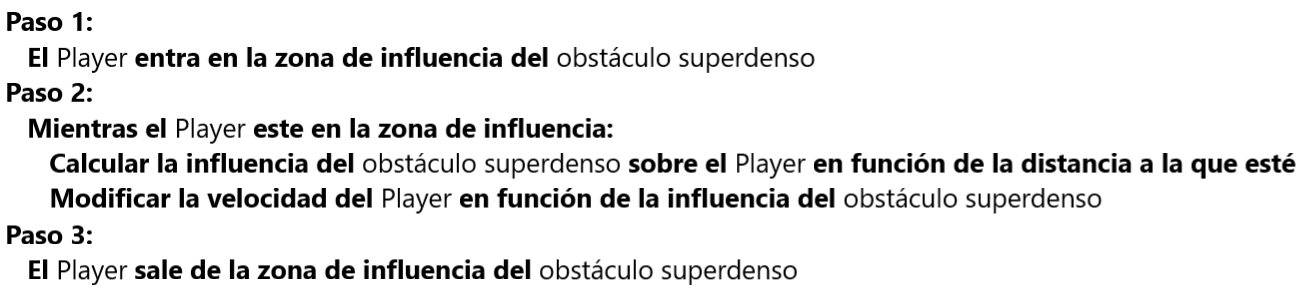
\includegraphics[scale=0.6]{Anexos/Anexo_C/Psuedocodigo_superdenso}
\caption{Pseudocódigo que resume el funcionamiento del obstáculo superdenso}
\end{figure}

\subsubsection{Inversor de gravedad}

\begin{figure}[h]
\centering
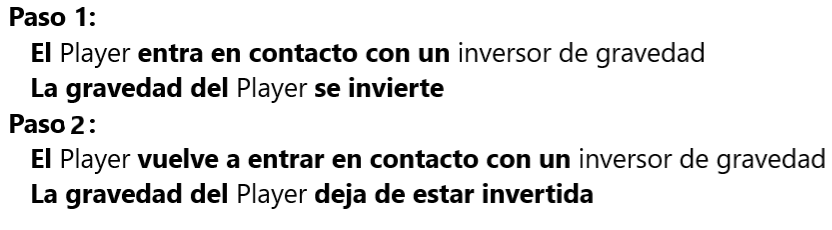
\includegraphics[scale=0.7]{Anexos/Anexo_C/Pseudocodigo_inversor}
\caption{Pseudocódigo que resume el funcionamiento del inversor de gravedad}
\end{figure}

\subsection{Movimiento de los obstáculos}
\subsubsection{Obstáculos estático}
Este obstáculo no se mueve.

\clearpage
\subsubsection{Obstáculos que siguen una rutina}

\begin{figure}[h]
\centering
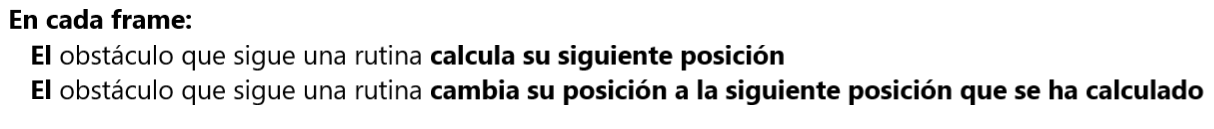
\includegraphics[scale=0.6]{Anexos/Anexo_C/Psudocodigo_rutina}
\caption{Pseudocódigo que resume el movimiento del obstáculo que sigue una rutina}
\end{figure}

\subsubsection{Obstáculos móviles}

\begin{figure}[h]
\centering
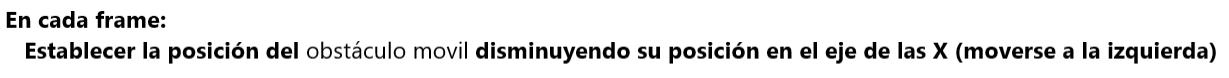
\includegraphics[scale=0.55]{Anexos/Anexo_C/Pseudocodigo_movil}
\caption{Pseudocódigo que resume el movimiento del obstáculo móvil}
\end{figure}

\subsection{Portales}
Para una de pareja de portales Portal1 y Portal2 enlazados entre sí.

\begin{figure}[h]
\centering
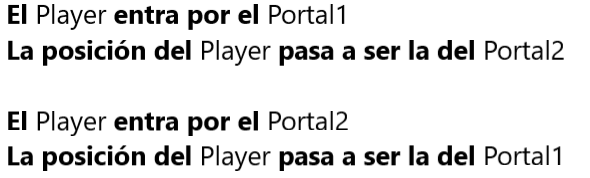
\includegraphics[scale=1]{Anexos/Anexo_C/Pseudocodigo_portal}
\caption{Pseudocódigo que resume el funcionamiento de los portales}
\end{figure}
\clearpage

\subsection{Creadores de impulso}
\subsubsection{Partícula de impulso}

\begin{figure}[h]
\centering
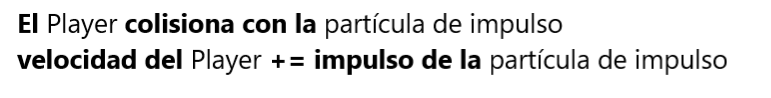
\includegraphics[scale=1]{Anexos/Anexo_C/Pseudocodigo_particula}
\caption{Pseudocódigo que resume el funcionamiento de la partícula de impulso}
\end{figure}

\subsubsection{Plataforma de salto}

\begin{figure}[h]
\centering
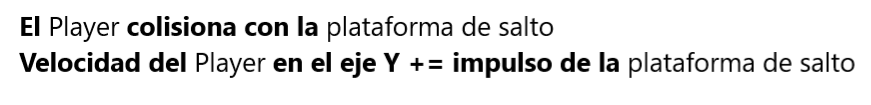
\includegraphics[scale=0.7]{Anexos/Anexo_C/Pseudocodigo_plataforma}
\caption{Pseudocódigo que resume el funcionamiento de la plataforma de salto}
\end{figure}

\subsubsection{Amplificador de impulso}

\begin{figure}[h]
\centering
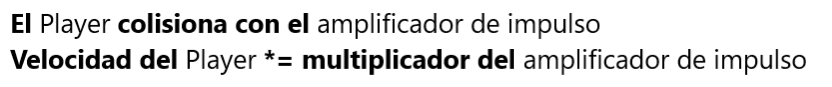
\includegraphics[scale=0.7]{Anexos/Anexo_C/Psudocodigo_ampificador}
\caption{Pseudocódigo que resume el funcionamiento del amplificador de impulso}
\end{figure}

\clearpage
\subsection{Animación de Sprites}
\subsubsection{SpriteAnimator}

\begin{figure}[h]
\centering
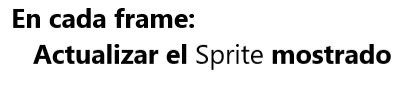
\includegraphics[scale=1]{Anexos/Anexo_C/Psudocodigo_loop_anim}
\caption{Pseudocódigo que resume el funcionamiento del animador en loop}
\end{figure}

\subsubsection{OneTimeAnimator}

\begin{figure}[h]
\centering
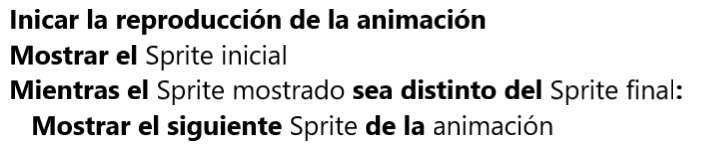
\includegraphics[scale=1]{Anexos/Anexo_C/Psuedocodigo_animador}
\caption{Pseudocódigo que resume el funcionamiento del animador de un solo uso}
\end{figure}

\subsection{Modificadores temporales}
\subsubsection{Tiempo bala}

\begin{figure}[h]
\centering
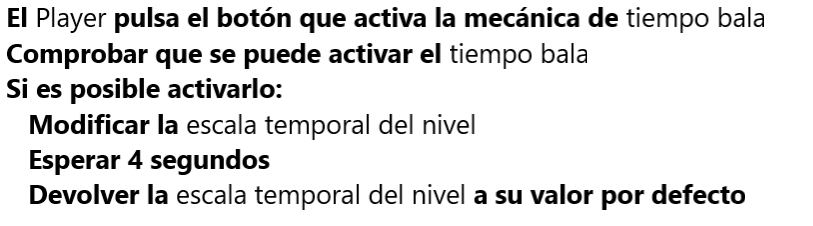
\includegraphics[scale=0.6]{Anexos/Anexo_C/Pseudocodigo_tiempo_bala}
\caption{Pseudocódigo que resume el funcionamiento de la mecánica de tiempo bala}
\end{figure}

\clearpage
\subsubsection{Zonas de gravitación temporal}

\begin{figure}[h]
\centering
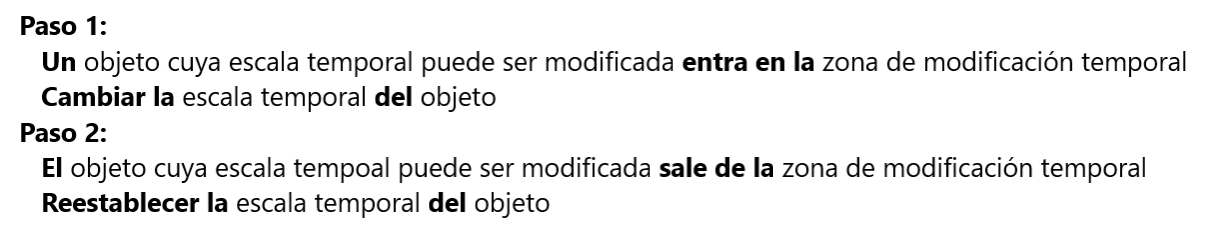
\includegraphics[scale=0.6]{Anexos/Anexo_C/Pseudocodigo_zona}
\caption{Pseudocódigo que resume el funcionamiento de las zonas de gravitación temporal}
\end{figure}

\section{Diseño de datos}
Los datos necesarios para el desarrollo de un videojuego son los Sprites y los audios utilizados durante su ejecución.

Para utilizar estos recursos en Unity se hace uso de los AudioSources \cite{AudioSource} y los SpriteRenderers \cite{SpriteRenderer}.

\subsection{AudioSource}
La clase AudioSource es la case de la que hace uso Unity para reproducir audios. Esta clase tiene un atributo público AudioClip que contendrá el audio que se va a reproducir. Se puede saber si el audio se esta reproduciendo con el atributo booleano isPlaying.\\
Se puede modificar el volumen de reproducción de todo audio reproducido con ese AudioSource.

Los métodos de reproducción de audios son los siguientes:
\begin{itemize}
\item
Play: reproduce el audio asociado al AudioSource (AudioSource.AudioClip).
\item
PlayDelayed: reproduce el audio asociado al AudioSource despues del tiempo pasado por parámetros.
\item
PlayOneShot: permite reproducir cualquier audio pasado como parámetro. El audio que se desea reproducir deberá estar encapsulado en una instancia de la clase AudioClip \cite{AudioClip} .
\end{itemize}

En el proyecto desarrollado AudioSource se ha usado para controlar el volumen del juego. Se ha creado una clase VolumeManager encargada de guardar y modificar el volumen general del juego y el volumen de la música.\\
Sin embargo, los AudioSources del juego están protegidos por clases envoltorio encargadas de modificar el volumen del juego de acuerdo a las opciones de juego.

\begin{figure}[h]
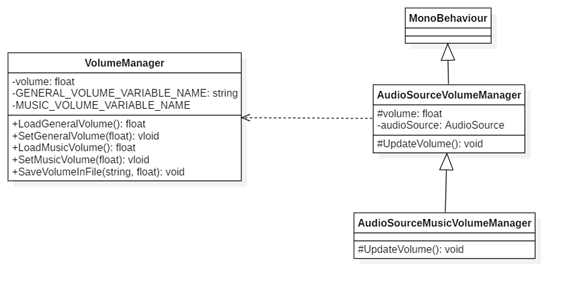
\includegraphics[scale=1]{Memoria/Aspectos_relevantes/Volumen_persistente/VolumeManager_UML}
\caption{Diagrama UML de las clases que hacen uso del AudioSource}
\end{figure}

\subsection{SpriteRenderer}
La clase SpriteRenderer es la encargada de hacer que se muestre una imagen en una zona del videojuego. Para poder mostrar las imágenes en Unity hay que utilizar la clase envoltorio Sprite. SpriteRenderer tiene un atributo público Sprite que contiene la imagen que mostrará ese SpriteRenderer.

En el proyecto se ha hecho uso de esta clase para mostrar imágenes estáticas y para mostrar animaciones.\\
Para crear las animaciones se ha creado dos clases SpriteAnimator y OneTimeAnimator. Estas clases simulan la animación intercalando a grandes velocidades un conjunto de imágenes. La diferencia entre estas dos clases es que SpriteAnimator reproduce una animación indefinidamente en bucle y OneTimeAnimator reproduce la animación una sola vez.

\begin{figure}[h]
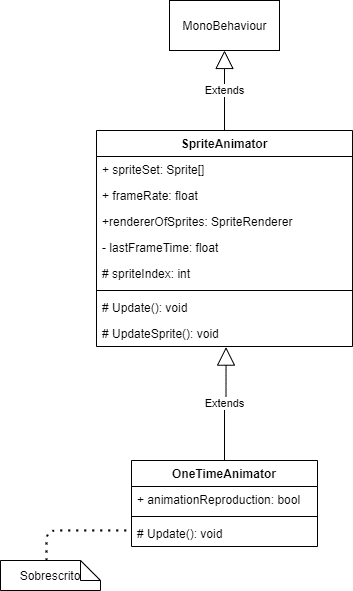
\includegraphics[scale=0.8]{Memoria/Aspectos_relevantes/Animadores/Herencia_animators}
\caption{Diagrama UML de las clases SpriteAnimator y OneTimeAnimator}
\end{figure}

\section{Diseño procedimental}
En este apartado se explicarán los algoritmos que se han desarrollado para el correcto funcionamiento del videojuego.

\subsection{Sistema de colisiones}
Para simular el sistema de colisiones se optó por utilizar la velocidad como elemento principal.

\clearpage
\begin{figure}[h]
\centering
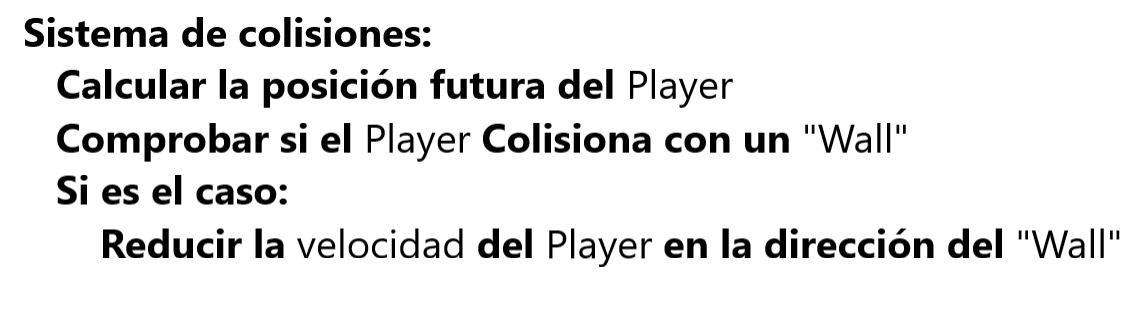
\includegraphics[scale=0.7]{Anexos/Anexo_C/Pseudocodigo_colisiones}
\caption{Pseudocódigo que resume el sistema de colisiones}
\end{figure}

Para saber si un KinematicObject va a colisionar con el suelo o un muro (se identifican los objetos con los que se desea chocar porque tienen asignada la layer “Wall”) se coge la velocidad del KinematicObject (se obtiene del atributo velocity del Rigidbody2D), que está representada en unidades/segundo. Con la velocidad que lleva el KinematicObject y su posición se puede deducir la siguiente posición en la que se encontrará.

Hay un método que se llama Physics2D.BoxCast con el que puedes crear un rectángulo en una región del espacio y comprobar si se colisiona con algún objeto. En caso de colisionar con un objeto se devuelve un objeto de la clase RayCastHit2D con toda la información relativa a la colisión. Hay un método similar a Physics2D.BoxCast que es Physics2D.BoxCastAll que hace lo mismo pero devolviendo un vector de RayCastHit2D con un elemento por cada objeto con el que has colisionado.

Se puede filtrar las colisiones por Layer, pudiendo solo tener en cuenta las colisiones con objetos que tengan asociada una Layer con el mismo nombre que el pasado por parámetro en el método. Para el sistema de colisiones solo se han tenido en cuenta los objetos con Layer igual a “Wall”.

Con el método Physics2D.BoxCastAll se va a crear un rectángulo del tamaño del Collider2D del KinematicObject en la siguiente posición en la que se encontrará el objeto y comprobarán cuántos objetos con Layer igual a “Wall” colisionarán en esa posición con el KinematicObject.

\clearpage
\begin{figure}[h]
\centering
\includegraphics[scale=1]{Memoria/Aspectos_relevantes/Sistema_Colisiones/Detección_colisiones}
\caption{Simulación del proceso de detección de colisiones}
\end{figure}

Una vez detectados con que muros se han colisionado (objetos con Layer igual a “Wall”) se va a simular el choque modificando la velocidad del KinematicObject poniendo a cero la velocidad en la dirección de la colisión del muro. Un ejemplo de aplicación sería un KinematicObject yendo a una velocidad marcada por el vector (1, -2), es decir 1 unidad hacia la derecha (eje x) y dos unidades hacia abajo (eje y). Si se detecta que se va a colisionar contra el suelo (un muro que está a los pies del KinematicObject) la velocidad debería establecerse al vector (1,0), es decir continuar el desplazamiento a la derecha pero cesar el movimiento hacia abajo.

Para calcular en qué dirección hay que limitar la velocidad se utiliza el vector normal de la recta creada por la pared más cercana del muro. Ese vector normal lo ofrece el objeto RayCastHit2D en su atributo “normal”.
Se va a añadir una figura explicativa:

\clearpage
\begin{figure}[h]
\centering
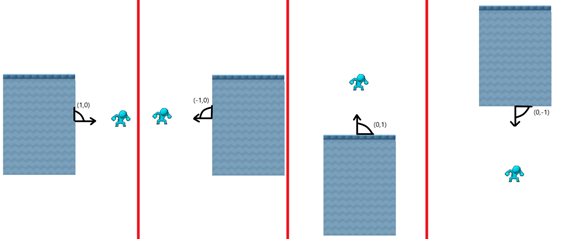
\includegraphics[scale=1]{Memoria/Aspectos_relevantes/Sistema_Colisiones/Vector_normal}
\caption{Vector normal del muro en función de la posición del KinematicObject}
\end{figure}

De la colisión del KinematicObject se encarga el objeto KinematicObjectCollisionManager, que tiene una referencia a KinematicObject y se encarga de llamar al método Physics2D.BoxCastAll y limitar la velocidad del KinematicObject en caso de colisión.

\begin{figure}[h]
\centering
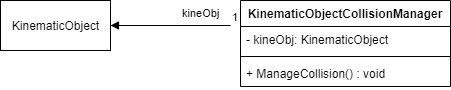
\includegraphics[scale=1]{Memoria/Aspectos_relevantes/Sistema_Colisiones/KinematicObjectCollisionManager_UML}
\caption{Diagrama UML del sistema de colisiones}
\end{figure}

\subsection{Modificaciones gravitatorias}
Los objetos kinemáticos pueden recibir modificaciones gravitatorias que alteren su velocidad. De esta labor se encarga la clase KinematicObjectGravityManager.\\
Esta clase tiene una lista con todas las alteraciones gravitatorias que se aplicarán en ese loop del FixedUpdate. En cada loop del FixedUpdate se aplicarán al KinematicObject asociado a esa instancia de KinematicObjectGravityManager y se vaciará la lista.

\begin{figure}[h]
\centering
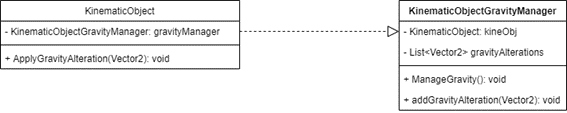
\includegraphics[scale=1]{Memoria/Aspectos_relevantes/Modificaciones_gravitatorias/KinematicObjectGravityManager_UML}
\caption{Diagrama UML de la clase encargada de la gestión de la gravedad del KinematicObject}
\end{figure}

\begin{figure}[h]
\centering
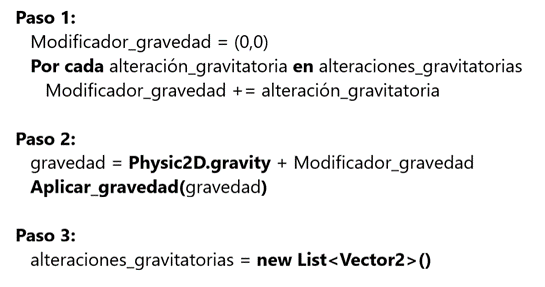
\includegraphics[scale=1]{Memoria/Aspectos_relevantes/Modificaciones_gravitatorias/Pseudocodigo_modificadores_gravedad}
\caption{Pseudocódigo del proceso de modificación de la gravedad del KinematicObject en cada loop del FixedUpdate}
\end{figure}

\subsection{TimeAffectedObjects}
Hay una serie de objetos que se ven afectados por las modificaciones temporales particulares. Estos objetos heredarán de la clase TimeAffectedObject. 

\begin{figure}[h]
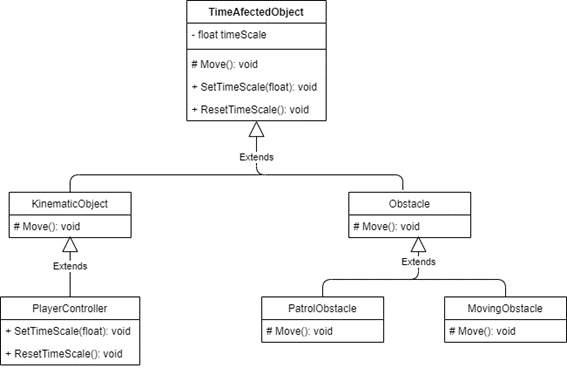
\includegraphics[scale=1]{Memoria/Aspectos_relevantes/Tiempo_bala/Herencia_TimeAffectedObject}
\caption{Clases que heredan de TimeAffectedObject}
\end{figure}

El movimiento de las clases que hereden de esta deberá implementarse en el método Move, pues será en ese método en el que se aplicará la modificación temporal al movimiento acelerándolo o ralentizándolo según toque.

Cuando el juego vuelva al estado inicial será necesario restablecer la escala temporal de todos los TimeAfectedObjects a la escala por defecto.

\begin{figure}[h]
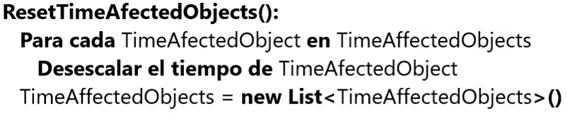
\includegraphics[scale=1]{Memoria/Aspectos_relevantes/Tiempo_bala/Pseudocodigo_TimeAffectedObject}
\caption{Pseudocódigo del método llamado para resetear los TimeAfectedObject}
\end{figure} 

\section{Diseño arquitectónico}
\subsection{GameController}
Se ha desarrollado una arquitectura específica para asegurar que los niveles jugables tienen están siempre en un estado estable de juego, y un proceso a seguir cada vez que se reinicia el nivel a su estado inicial.\\
Con este propósito se ha creado la clase GameController. Esta clase contiene dos elementos distintos al servicio del mismo propósito.

\begin{figure}[h]
\centering
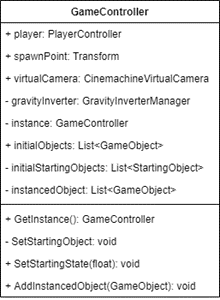
\includegraphics[scale=1]{Memoria/Aspectos_relevantes/GameController/GameController}
\caption{Diagrama UML de la clase GameController}
\end{figure}

\subsection{Variables de PlatformerModel}
La clase GameController contendrá una serie de atributos que, al iniciar la escena copiará en la clase PlatformerModel esos atributos. Estas variables son variables relevantes del nivel. Son movidas a la clase PlatformerModel para que todos los objetos de la escena puedan acceder a estas variables facilmente sin generar cadenas de mensajes para tener acceso a ellas.

Las variables de GameController que serán copiadas a PlatformerModel serán:
\begin{itemize}
\item
La CinemachineVirtualCamera que utiliza la escena (PlatformerModel.virtualCamera).
\item
El PlayerController asignado al avatar jugable (PlatformerModel.player).
\item
El objeto de tipo Transform asociado al punto de reaparición e inicio de escena del Player (PlatformerModel.spawnPoint).
\item
El GameController de la escena (PlatformerModel.gameController).
\item
El GravityInverterManager asociado a la escena \\ (PlatformerModel.gravityInverterManager).
\end{itemize}

\subsection{Estado inicial de juego}
Cuando el Player muera será necesario devolver el nivel al estado inicial en el que se encontraba al acceder a esa escena.\\
Para volver a este estado inicial será necesario:
\begin{itemize}
\item
Eliminar los objetos creados que no estaban instanciados al inicio del nivel.
\item
Devolver los objetos cuyo estado haya variado durante la ejecución del nivel a su estado inicial (un ejemplo sería devolver un obstáculo que sigue una rutina del punto en el que se encuentra al punto en el que empieza el juego).
\item
Instanciar objetos que estaban al inicio del nivel pero que ya no están instanciados.
\item
Devolver el Player a su posición inicial.
\end{itemize}

En la implementación del programa, se han tratado todos los objetos que debían ser devueltos a su estado inicial (salvo al Player) como el mismo tipo de objetos. Han sido guardados en una clase envoltorio que guarda el estado inicial del objeto. Estos objetos no serán los que estén en la escena, sino que en el estado inicial del juego se generarán clones de él en la escena.\\
Todos los objetos instanciados serán guardados en la lista instancedObjects para poder destruirlos cuando haya que reiniciar el nivel. Los objetos que se instancien durante la escena también serán añadidos a isntancedObjects.

\clearpage
\begin{figure}[h]
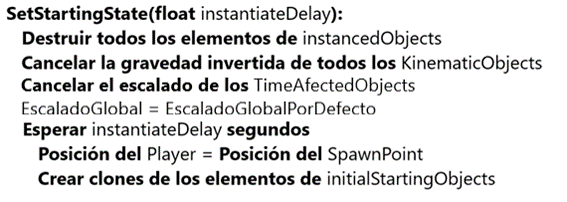
\includegraphics[scale=1]{Memoria/Aspectos_relevantes/GameController/Pseudocodigo_starting_objects}
\caption{Pseudocódigo de las operaciones realizadas al establecer el estado inicial del nivel}
\end{figure}

\subsection{Estados del Player}
El Player se comportará de distinta forma en función de en que situación se encuentre. Para facilitar la lógica del Player y el cambio en tiempo de ejecución del comportamiento de este, se ha aplicado el patrón de diseño Estado.

\begin{figure}[h]
\centering
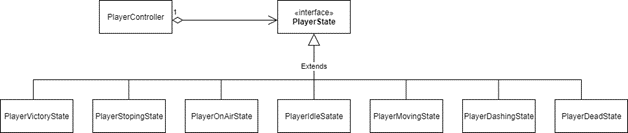
\includegraphics[scale=0.85]{Memoria/Aspectos_relevantes/Arquitectura_Player/Estados_Player}
\caption{Diagrama UML de la aplicación del patrón de diseño Estado en el Player}
\end{figure}

El Player puede estar en los siguientes estados:
\begin{itemize}
\item
PlayerIdleState: El Player está detenido sobre una superficie.
\item
PlayerOnAirState: El Player está en el aire.
\item
PlayerMovingState: El Player se está moviendo sobre una superficie.
\item
PlayerStopingState: El Player ha cesado el movimiento y se está deteniendo.
\item
PlayerDashingState: El Player está realizando el acelerón.
\item
PlayerVictoryState: El Player ha llegado a la meta.
\item
PlayerDeadState: El Player está muerto.
\end{itemize}

\begin{figure}[h]
\centering
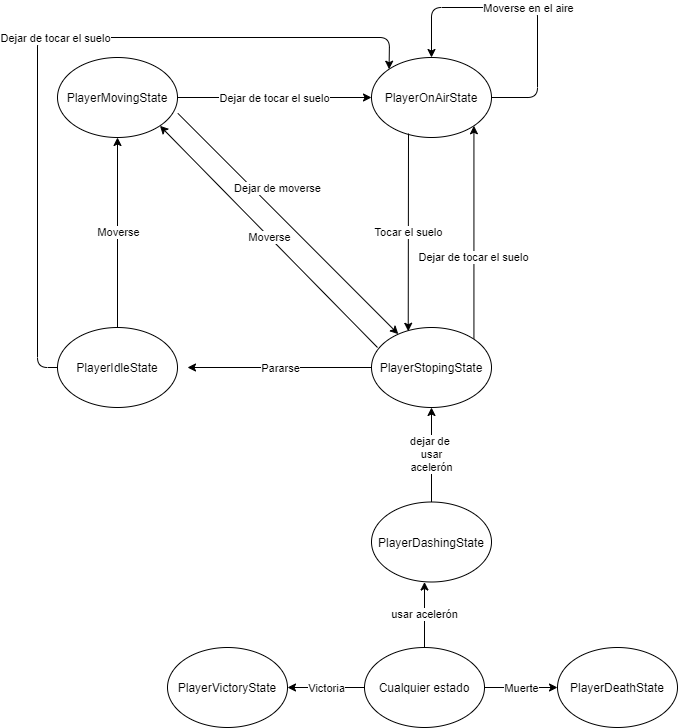
\includegraphics[scale=0.55]{Memoria/Aspectos_relevantes/Arquitectura_Player/Diagrama_de_estados}
\caption{Diagrama de transición entre estados del Player}
\end{figure}